\chapter{Stochastic RL-MPC}
\label{chapter:stochastic_RL_MPC}

This chapter outlines the performance gains of various RL-MPC implementations as selected from \autoref{chapter:deterministic_RL_MPC} in a stochastic environment. The initial performances of the standalone RL agents and MPC in various levels of uncertainty will be investigated followed by comparisons with the RL-MPC implementations. This chapter seeks to demonstrate the effectiveness of RL-MPC controllers in a realistic setting, providing insight into the controller's potential performance in real-world applications.

\section{Initial RL and MPC Performance}5

\begin{figure}[H]
	\centering
	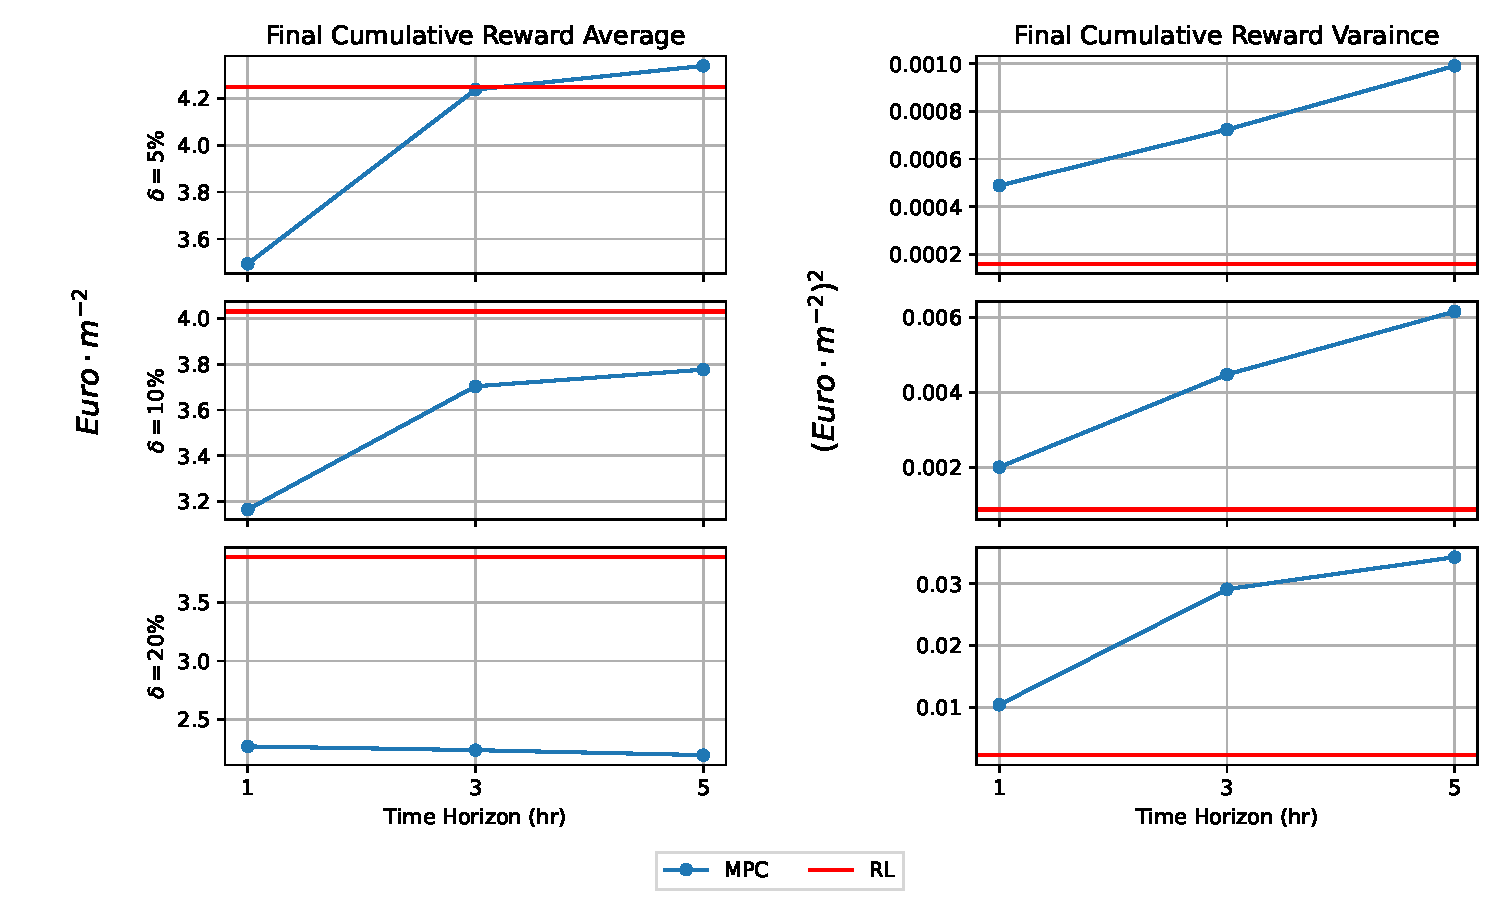
\includegraphics[width=\textwidth]{figures/stochastic_rl_vs_mpc.eps}
	\caption{RL vs MPC in stochastic conditions}
	\label{fig:stochastic-rl-vs-mpc}
\end{figure}

\emph{The initial performances of the respective MPC and RL performances}

\section{Results - Implementation 3}
\emph{Results of including the vf from the trained agent, a self-trained vf and initial guesses from actor, and then finally a reduced order self-trained vf}

\begin{figure}[H]
	\centering
	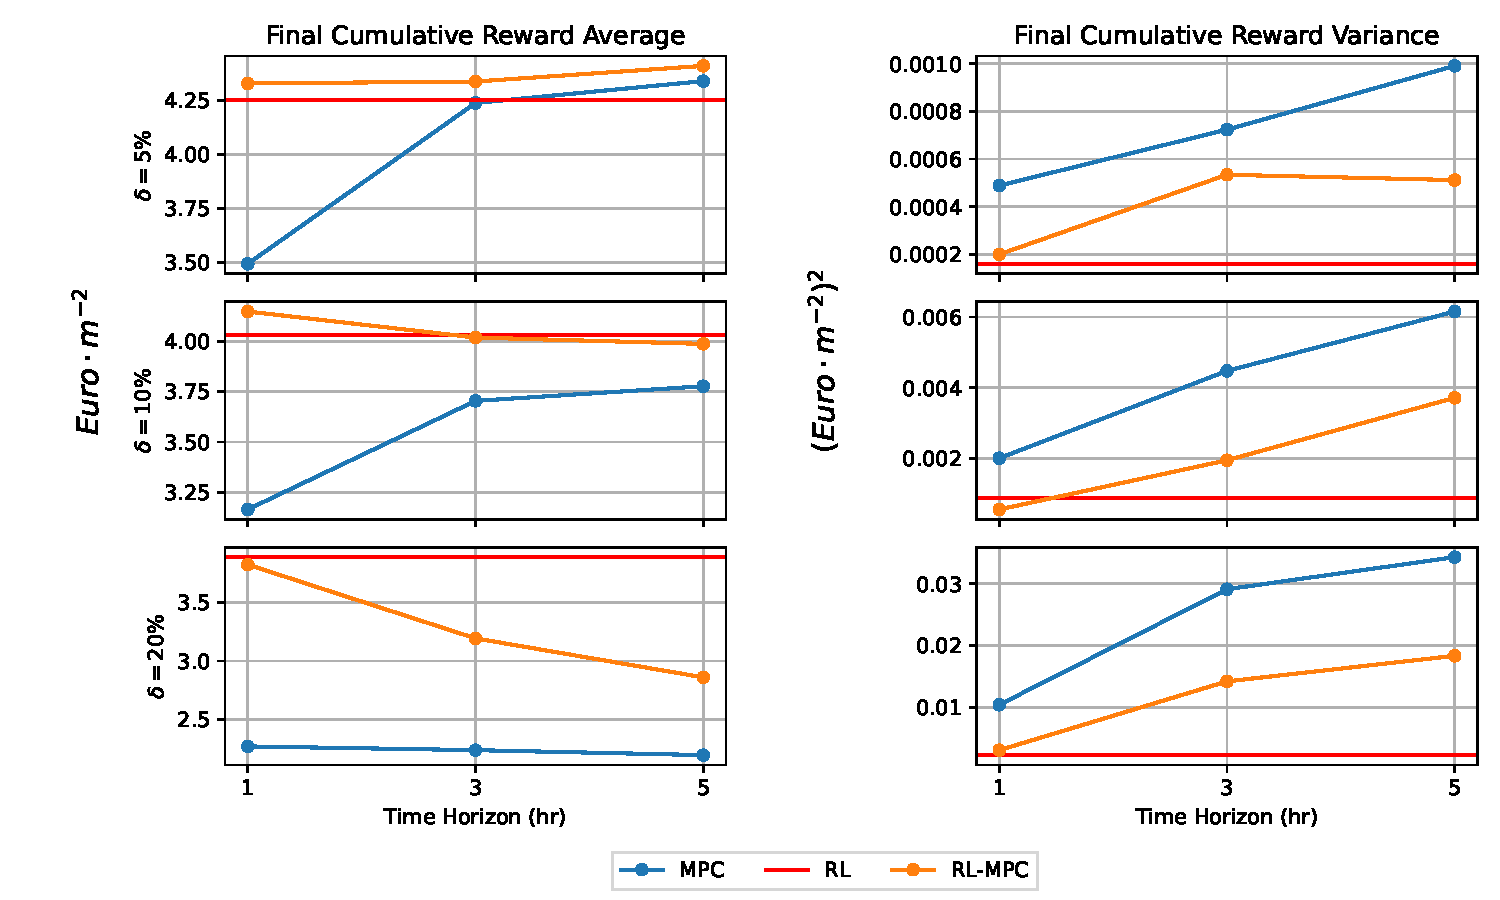
\includegraphics[width=\textwidth]{figures/stochastic_rl_vs_mpc_impl3.eps}
	\caption{MPC vs stochastic RL-MPC Impl3}
	\label{fig:stochastic-rlmpc-impl3}
\end{figure}

\begin{figure}[H]
	\centering
	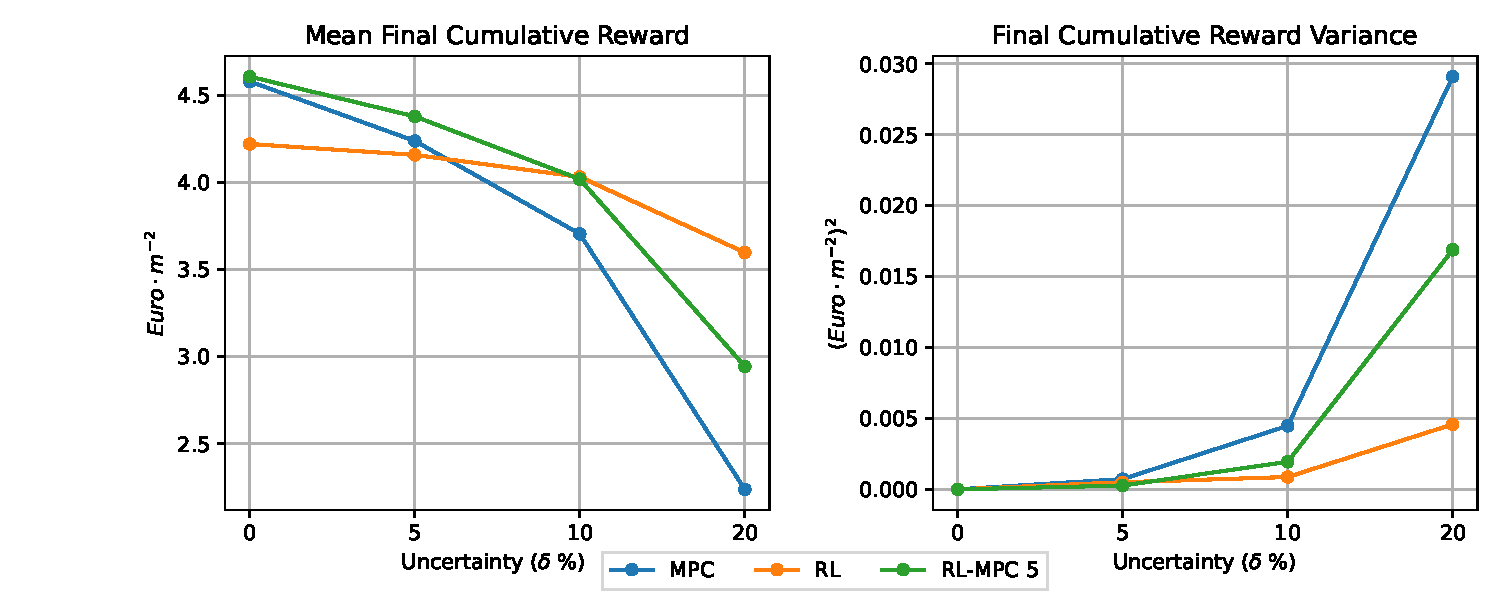
\includegraphics[width=\textwidth]{figures/stochastic_realife.eps}
	\caption{MPC vs RL vs RL-MPC}
	\label{fig:stochastic-reallife}
\end{figure}

\section{Results - Implementation 5}
\emph{The Results and discussion of combining the two}


\section{Final Result and Conclusion}
\emph{The final selected algorithm and conlusion on the work done}